\documentclass[]{report}

\usepackage{import}

\import{../}{settings.tex}

\title{Cours de probabilité pour l'agrégation}

\author{Cours de Mathieu Merle, transcrit par SADR TAHOURI Luca}
\date{}



\begin{document}

    \maketitle
    \tableofcontents

\chapter{Espaces mesurés}

\section{Introduction}

La théorie de la mesure fournit un cadre mathématique commun pour
\begin{itemize}
    \item Notions classiques de mesure (distance, aire, volume) et les intégrales associées
    \item Formalisation et quantification d'expériences aléatoires.
    \begin{itemize}[label=$\hookrightarrow$]
        \item Expérience dont le résultat est imprévisible.
        \item Quantités moyennées
    \end{itemize}
\end{itemize}

\begin{ex}{}{}
    \begin{enumerate}
        \item "Temps" du vainqueur du $100m$ e.g. aux J.O.\\
        Ce qu'on peut mesurer dépend de la précision de l'appareil de mesure.\\
        Avec un chronomètre au 10e de seconde, $T$ étant le temps du vainqueur,
        \[\text{L'évènement } \cho{\left\{ T\le 10\right\}\text{ est mesurable}\\ \text{mais }\left\{10,24\le T\le 10,28\right\}\text{ ne l'est pas} }\]
        \item (Exo 2 du TD) Une contient $b$ boules bleues et $r$ boules rouges.\\
        Tirages uniformes, successifs, sans remise. Pour $k\ge 1$
        \[\Pa\left(\text{1er rouge soit tirée lors du $k$e tirage}\right)=\dfrac{b}{b+r}\dfrac{b-1}{b+r-1}\ldots \dfrac{b-k+2}{b+r-k+2}\dfrac{r}{b+r-k+1}\]
        \item mesure de l'aire cultivable d'un champ rectangulaire, au milieu duquel se trouve une mare
        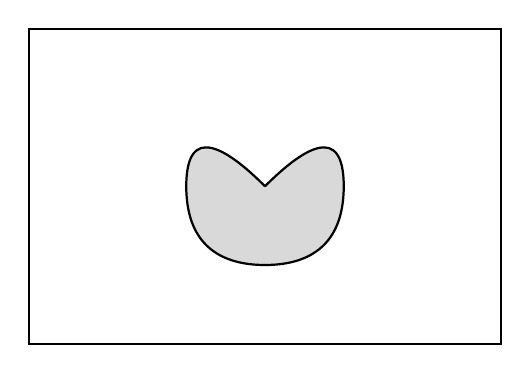
\begin{tikzpicture}
    % Dessiner le rectangle
    \draw[thick] (0,0) rectangle (6,4);

    % Dessiner la mare au centre (forme plus organique et réaliste)
    \draw[thick, fill=gray!30] (3,2) .. controls (2.5,2.5) and (2,2.8) .. (2,2)
                              .. controls (2,1.2) and (2.5,1) .. (3,1)
                              .. controls (3.5,1) and (4,1.2) .. (4,2)
                              .. controls (4,2.8) and (3.5,2.5) .. (3,2);
\end{tikzpicture}
    \end{enumerate}
\end{ex}

\section{Tribus, mesures, exemples fondamentaux, caractérisation d'une mesure de probabilité}

$\Omega$ un ensemble quelconque, qu'on appelle "Univers"

\begin{df}{Tribu et espace mesurable}{}
    $\Fr\subset \Par(\Omega)$ est une tribu sur $\Omega$ si
    \begin{enumerate}[label=\roman*]
        \item $\Omega\in \Fr$
        \item $A\in \Fr\implies A^C\in \Fr$
        \item $(A_n)\subset \Fr\implies \bigcup_{\nN} A_n\in \Fr$
    \end{enumerate}
    On appelle $(\Omega,\Fr)$ un espace mesurable
\end{df}

\begin{prop}{}{}
    \begin{enumerate}[label=\alph*]
        \item $\emptyset\in \Fr$
        \item $A_1,\ldots,A_n\in \Fr$ alors $\bigcup_{i\in \llbracket 1,n\rrbracket} A_i \in \Fr, \bigcap_{i\in \llbracket 1,n \rrbracket} A_i \in \Fr$
        \item $A,B\in \Fr, B\wt A\in \Fr, A \qquad A\triangle B=(A\cup B)\wt (A\cap B)\in \Fr$
        \item $(A_n)\in \Fr^\N,\limsup A_n=\bigcap_n \bigcup_{p\ge n}A_p\in \Fr,\liminf A_n=\bigcup_n \bigcap_{p\ge n} A_p$
    \end{enumerate}
\end{prop}

\begin{df}{Mesure positive, espace mesuré, mesure $\sigma$-finie, mesure de probabilité, espace probabilisé}{}
    $\mu$ mesure positive sur $(\Omega,\Fr)$ si $\funto{\mu}{ \Fr}{\R_+ \cup \{+\infty\}}$ tq
    \begin{enumerate}[label=\roman*]
        \item $\mu (\emptyset)=0$
        \item $(A_n)_\nN\in \Fr^\N$ 2 à 2 disjoints,
        \[ \mu \left( \bigcup_\nN A_n \right)=\sum_\nN \mu(A_n)\]
    \end{enumerate}
    On dit que $(\Omega,\Fr,\mu)$ est un espace mesuré
    \begin{itemize}
        \item Si $\exists (\Omega_n)\nearrow$ tq $\bigcup_\nN \Omega_n=\Omega$, $\mu(\Omega_n)<+\infty,\forall n\in \N$, on dit que $\mu $ est $\sigma$-finie.
        \item Si $\mu(\Omega)=1$, on dit que $\mu$ est une probabilité, et alors $(\Omega,\Fr,\mu)$ est un espace probabilisé.
    \end{itemize}
\end{df}

\begin{prop}{}{}
    \begin{enumerate}[label=\alph*]
        \item $A_1,\ldots,A_n\in \Fr$, 2 à 2 disjoints
        \[ \mu\left( \bigcup_{k=1}^n A_k\right)= \sum_{i=1}^n \mu (A_i)\]
        \item \[\forall A,B\in \Fr,\mu(a)+\mu(B)=\mu(A\cup B)+ \mu(A\cap B)\]
        \item \[A\subset B, A,B\in \Fr, \mu(A)\le \mu(B)\]
        et si $\mu(A)<+\infty, \mu(B\wt A)=\mu(B)-\mu (A)$\\
        $(A_n)\in \Fr^\N,\mu(\bigcup_\nN A_n)\le \sum_{\nN} \mu(A_n)$
        \item $(A_n)\in \Fr^\N \nearrow,\mu\left(\bigcup A_n\right)=\lim \mu(A_n)$\\
        $(A_n)\in \Fr^\N \searrow,\mu\left(\bigcap A_n\right)=\lim \mu(A_n)$
    \end{enumerate}
\end{prop}

\begin{prop}{}{}
    \begin{enumerate}[label=\alph*]
        \item Si $\forall i\in I,\Fr_i$ est une tribu sur $\Omega$, alors $\bigcap_{i\in I}\Fr_i$ est une tribu sur $\Omega$
        \item $\Ar\subset \Pr(\Omega)$, on note $\sigma(A)$ et on appelle tribu engendrée par $\Ar$,
        \[\sigma(A):=\bigcap_{\substack{\Fr \text{ tribu sur $\Omega$}\\  \Ar\subset \Fr}} \Fr\]
        L'intersection est non vide car $\Par(\Omega)$ est une tribu sur $\Omega$ et $\sigma(A)$ est la plus petite tribu sur $\Omega$ contenant $\Ar$
    \end{enumerate}
\end{prop}

\begin{df}{Tribu des Boréliens}{}
    Si $\Omega$ est un espace topologique, $\Br(\Omega)$ la tribu des boréliens de $\Omega$ est
    \[\Br(\Omega)=\sigma\left(\left\{\text{ouverts de $\Omega$}\right\}\right)\]
\end{df}

\begin{df}{Tribu produit}{}
    $(E,\Ar),(\Fr,\Br)$ espaces mesurables
    \[\Ar\otimes \Br := \sigma \left(\left\{A\times B,A\in \Ar,B\in \Br\right\}\right)\]
    est la tribu produit
\end{df}

\begin{prop}{}{}
    \[\Br(\R)^{\otimes d}=\Br (\R^d)\]
\end{prop}

\begin{df}{Mesure produit}{}
    $(E,\Ar,\mu),(F,\Br,\nu)$ espaces mesurés, alors
    \[\funto{\mu \otimes \nu}{\Ar\otimes \Br}{\R_+\cup \{+\infty\}}\]
    l'unique mesure telle que $\forall A\in \Ar,B\in \Br$
    \[\mu\otimes \nu(A\times B)= \mu(A)\times \nu (B)\]
\end{df}

\begin{tm}{Existence et unicité de la mesure de Lebesgue}{}
    Il existe une unique mesure sur $(\R,\Br(\R))$, notée $\lambda$ et appelée mesure de Lebesgue telle que
    \[\lambda\left(]a,b[\right)=b-a,\forall (a,b)\in \R^2\]
    Il existe une unique mesure $\lambda_d$ sur $\left(\R^d,\Br(\R^d)\right)$ telle que
    \[\lambda\left(\produit{i=1}{d} ]a_i,b_i[\right))\produit{i=1}{d}(b_i-a_i)\]
    \begin{itemize}
        \item De plus, $\lambda_d=\lambda^{\otimes d}$
        \item $\lambda_d$ est aussi l'unique mesure sur $\left(\R^d,\Br(\R^d)\right)$ invariante par translation telle que $\lambda_d\left([0,1]^d\right)=1$
    \end{itemize}
\end{tm}

\begin{prop}{}{}
    $\funto{f}{\Omega}{E}$ et $\Gr$ tribu sur $E$. On note
    \[f^{-1}(\Gr):=\left\{f^{-1}(B),B\in \Gr\right\}\]
    C'est une tribu sur $\Omega$. On l'appelle la tribu "Image réciproque" de $\Gr$ par $f$.\\
    Si $\Fr$ est une tribu sur $\Omega$,
    \[f^{\to}(\Fr):=\left\{B,f^{-1}(B)\in \Fr\right\}\]
    C'est une tribu sur $E$. On l'appelle "tribu image directe" de $\Fr$ par $f$\\
    Si $(\Omega,\Fr,\mu)$ espace mesuré, on peut définir $\mu_f$ ou $\mu\circ f$ la mesure image de $\mu$ par $f$,
    \[\fundfto{\mu_f}{f^{\to}(\Fr)}{\R_+\cup \{+\infty\}}{B}{\mu(f^{-1}(B))}\]
\end{prop}

\section{Dénombrement: exemples formalisés de probabilités discrètes}

\section{Indépendance d'évènements, de tribus, Borel-Cantelli, loi du $0-1$}

\chapter{Variables aléatoires}

\chapter{Convergence d'une suite de variables aléatoires et Théorèmes limites}

\chapter{Statistique}
\end{document}